\documentclass{article}

% Course instructions replace conference rules (names shown with the preprint option; no checklist).
\usepackage[preprint]{neurips_2026}

\usepackage[utf8]{inputenc}
\usepackage[T1]{fontenc}
\usepackage{hyperref}
\usepackage{url}
\usepackage{booktabs}
\usepackage{amsfonts}
\usepackage{nicefrac}
\usepackage{microtype}
\usepackage{xcolor}
\usepackage{graphicx}
\usepackage{tikz}
\usepackage{pgfplots}
\usepackage{enumitem}
\pgfplotsset{compat=1.17}
\usetikzlibrary{positioning,arrows.meta,calc}
\setlist{nosep,leftmargin=1.4em}

% Visible markers for things only a teammate can fill in or confirm; none may survive into the final PDF.
\newcommand{\todo}[1]{\textcolor{red}{[TODO: #1]}}
\newcommand{\fac}{Fa\c{c}ade}

\title{Fragile: A Trainable Drama Manager\\for a Turn-Based Interactive Mystery}

\author{%
  Qinchuan Zhang \qquad Haosen Cao \qquad Haorui Li \\
  Jingrui Ye \qquad Daolong Yang \qquad Zhonghui Chen \\[1mm]
  University of Southern California \\
  CSCI 566 Project Midterm Report \quad Group 26 \quad Fall 2026
}

\begin{document}

\maketitle

\begin{abstract}
\fac{} showed that an interactive drama can be steered by a drama manager that picks the next authored story beat, but its authors estimated two person-years of hand-writing for twenty minutes of play, and beat selection rested on hand-set weights, priorities and a match to a tension arc. Fragile is a turn-based interactive mystery in the \fac{} lineage: each turn the player writes what they say and do, a drama manager picks the next authored beat, an LLM performs it, and a guard model checks the result. Four modules (beat scoring, input understanding, consistency checking, tension estimation) each have a rule path and an LLM path, and a slot for a trained path. At the midpoint we report (i) a complete, playable system with 20 authored beats; (ii) a self-play pipeline in which LLM players with HEXACO-sampled personalities play whole sessions through the engine; (iii) a prefix-blind pairwise annotation protocol; and (iv) first results from 11 complete sessions (297 turns, \$0.22 per session). The LLM paths clearly beat the rule paths on small hand-written test sets. The drama manager, however, rarely has a real decision to make: the median probability of its top candidate is 0.98, and only 42\% of scored decisions offer two or more authored candidates. Reading the eight pilot transcripts exposed repeated and unresponsive character lines; one fix lowers a duplicated question in the opening from 7 of 8 openings to 0 of 8. No trained scorer exists yet. We describe what blocks it and our plan for the remaining two weeks.
\end{abstract}

\section{Introduction}

\fac{}~\citep{mateas2003facade,mateas2005structuring} is still the touchstone for interactive drama: a player who types natural language becomes entangled in the collapsing marriage of an AI-driven couple, while an invisible drama manager chooses the next \emph{beat}, a short unit of dramatic action, so that story tension follows an Aristotelian arc. Its cost was authorial. The authors expected to spend two man-years writing behaviours for a twenty-minute one-act play that could be replayed six or seven times before it was exhausted~\citep{mateas2003facade}, and beat selection rested on author-set weights and priorities plus the match between a beat's tension effect and an author-specified arc~\citep{mateas2005structuring}. Large language models now make it possible to attack that bottleneck directly: they can perform a beat from its dramatic intent, understand free-form input, and check a passage for contradictions. What they do not give us is a drama manager whose taste can be \emph{learned}.

Fragile tests that idea in one scene built on the skeleton of Hitchcock's \emph{Rope}. On the night before Julian and Mia emigrate, the player, an old college friend, comes to their farewell dinner, served on a shipping crate in an emptied flat. Leo, the friend they invited, never arrives; he is in the crate. The player writes one turn at a time, and the system answers with a first-person passage. The architecture keeps \fac{}'s beat abstraction but splits the drama manager into four modules, each with three interchangeable paths: a \emph{rule} baseline, a zero-shot \emph{LLM} path that plays the role of teacher, and a \emph{trained} student (Section~\ref{sec:system}). We ask four research questions.
\begin{description}
  \item[RQ1] Can LLM paths stand in for all four modules well enough to run a complete drama?
  \item[RQ2] Does a beat scorer learned from preference data follow the intended tension arc better than hand-set weights and priorities?
  \item[RQ3] Can free-form player input be mapped onto structured story state without breaking coherence, and can a small multilingual model learn that mapping?
  \item[RQ4] Can LLM self-play plus an LLM judge produce enough preference data, calibrated against a small amount of human annotation?
\end{description}
Relative to the pre-proposal, the interface changed from a 2D scene with animated portraits to a turn-based text game with inline illustrations, and the script changed from the restaurant scene to the present story. The drama manager itself is unchanged. This report is a status report, not a results paper: the system and data pipeline are complete, the LLM baselines are measured, and the trained scorer (M1) is not yet started because it waits on labels.

\section{Literature review}
\label{sec:related}

\paragraph{Interactive drama and drama management.}
Drama management goes back to Weyhrauch's search-based drama manager~\citep{weyhrauch1997guiding}, which scores whole story trajectories with an author-defined evaluation function, and to its application to the interactive fiction \emph{Anchorhead}~\citep{nelson2005searchbased}. \fac{} replaced search with a beat sequencer: among the unused beats whose preconditions hold, it draws at random, weighted, from the highest priority tier, favouring the beat whose tension effect best matches an author-specified Aristotelian arc~\citep{mateas2003facade,mateas2005structuring,mateas2002interactive}. Surveys~\citep{roberts2008survey,riedl2013interactive} and narrative planning~\citep{riedl2010narrative} frame the same problem as experience management. A second line reduces authoring by simulating characters: Prom Week and Comme il Faut~\citep{mccoy2011promweek,mccoy2014social}, Versu~\citep{evans2014versu}, and Bad News~\citep{ryan2016badnews}, which moves part of the manager's job to a human wizard. Fragile stays on the \fac{} side of this split (authored beats, an explicit manager), because beats give the learned scorer a small discrete action space and logs that annotators can read.

\paragraph{LLMs for interactive narrative and game mastering.}
Generative agents~\citep{park2023generative} give LLM characters memory and planning, but with no dramatic arc. For role-playing games, CALYPSO~\citep{zhu2023calypso} assists a human dungeon master and FIREBALL~\citep{zhu2023fireball} supplies game logs with structured state. Closer to our setting, \citet{wu2024roleplay} fine-tune an LLM to follow a plot chain; StoryVerse~\citep{wang2024storyverse} lets an LLM ``act director'' instantiate abstract plot acts; Drama Llama~\citep{sun2025dramallama} lets an LLM check natural-language trigger conditions of authored storylets, and Dramamancer~\citep{wang2025dramamancer} also builds on LLM-powered storylets. In the works we reviewed, the generator is prompted or fine-tuned and the choice among story units is made by prompting. We keep the generator frozen and make the \emph{choice} learnable.

\paragraph{Preferences, rewards and LLM judges.}
Pairwise comparisons are the natural label for ``which next beat is better'': the Bradley--Terry model~\citep{bradley1952rank} underlies reward models learned from human preferences~\citep{christiano2017deep,ouyang2022training}, and direct preference optimisation~\citep{rafailov2023direct} removes the reward-model step. LLM judges can stand in for humans at scale but show position, verbosity and self-preference biases~\citep{zheng2023judging}, which is why our judge is calibrated against human labels and kept on a different model family from the narrator (Section~\ref{sec:data}).

\paragraph{Simulated players and personality.}
HEXACO~\citep{ashton2007hexaco} has six trait domains; a meta-analysis~\citep{moshagen2019hexaco} gives their intercorrelations, which we use to sample plausible people rather than independent traits. LLMs can express assigned personality traits in text~\citep{jiang2024personallm}; we translate each sampled vector into a few concrete behaviour rules instead of numbers.

\paragraph{Small encoders and distillation.}
For input understanding (M2) we distil an LLM teacher~\citep{hinton2015distilling} into one multilingual encoder, mDeBERTa-v3~\citep{he2023debertav3}, with a head per output.

\section{System and progress so far}
\label{sec:system}

\paragraph{Story and beats.}
The pool has 20 authored beats (14 story beats, 1 satellite, 5 endings) made of 45 steps. A beat has preconditions, a weight, a tension effect, a duration in story minutes, a dramatic intent in plain language, steps delivered one per turn, \emph{mix-ins} that react to what the player just did, and branch outcomes. Steps may carry conditional lines resolved by the engine against the current state, so the narrator never sees a condition. A story clock fires events (Nora's text, her call, her arrival, the knock) independent of the player. The five endings are \texttt{bon\_voyage}, \texttt{the\_witness}, \texttt{open\_it}, \texttt{confession} and \texttt{second\_crate}.

\begin{figure}[t]
\centering
\resizebox{\linewidth}{!}{%
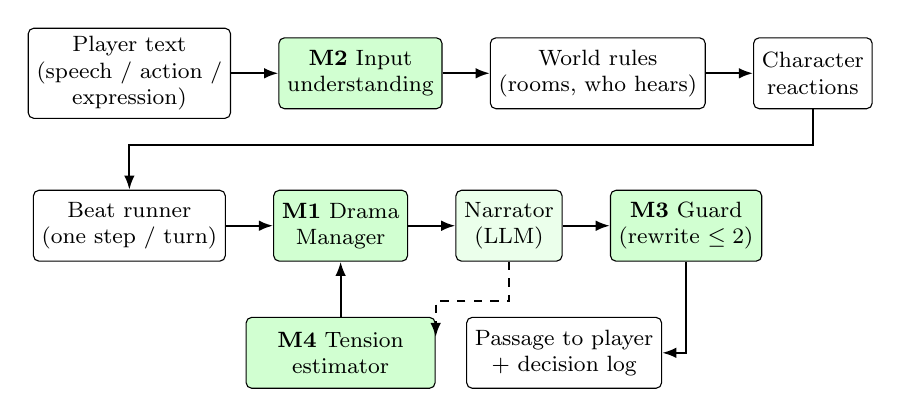
\begin{tikzpicture}[
  box/.style={draw, rounded corners=2pt, align=center, font=\footnotesize, minimum height=9mm, inner sep=3pt, fill=white},
  mod/.style={box, fill=green!18},
  llm/.style={box, fill=green!8},
  arr/.style={-{Latex[length=1.8mm]}, thick}]
  \node[box] (in) {Player text\\(speech / action /\\expression)};
  \node[mod, right=6mm of in] (m2) {\textbf{M2} Input\\understanding};
  \node[box, right=6mm of m2] (world) {World rules\\(rooms, who hears)};
  \node[box, right=6mm of world] (react) {Character\\reactions};
  \node[box, below=9mm of in] (run) {Beat runner\\(one step / turn)};
  \node[mod, right=6mm of run] (dm) {\textbf{M1} Drama\\Manager};
  \node[llm, right=6mm of dm] (narr) {Narrator\\(LLM)};
  \node[mod, right=6mm of narr] (guard) {\textbf{M3} Guard\\(rewrite $\le 2$)};
  \node[mod, below=7mm of dm, minimum width=24mm] (m4) {\textbf{M4} Tension\\estimator};
  \node[box, below=7mm of narr, xshift=7mm] (log) {Passage to player\\+ decision log};
  \draw[arr] (in) -- (m2); \draw[arr] (m2) -- (world); \draw[arr] (world) -- (react);
  \draw[arr] (react.south) -- ++(0,-4.5mm) -| ($(run.north)+(0,4.5mm)$) -- (run.north);
  \draw[arr] (run) -- (dm); \draw[arr] (dm) -- (narr); \draw[arr] (narr) -- (guard);
  \draw[arr] (m4) -- (dm);
  \draw[arr] (guard.south) |- (log.east);
  \draw[arr, dashed] (narr.south) -- ++(0,-5mm) -| ($(m4.east)+(0,2mm)$);
\end{tikzpicture}}
\caption{One turn. Shaded boxes are the four modules, each with a rule path, an LLM path (the teacher) and a slot for a trained path; the narrator is an LLM. The drama manager picks among the eligible beats at the highest priority tier plus a ``generate new beat'' option, sampling with $p(b)\propto \mathrm{score}(b)^{1/\tau}$. M4 reads the last four passages.}
\label{fig:arch}
\end{figure}

\paragraph{A turn and the four modules.}
Figure~\ref{fig:arch} shows the pipeline. \textbf{M2} turns free text into speech, action and expression channels, one of 27 dialogue acts per unit, addressee, topics, claims and an entry in a closed action table, and rejects inputs a player cannot decide (another character's actions, the outcome of an attempt, a convenient new object) with a suggested rewrite. Deterministic world rules decide where everyone is and who can hear the player. A bounded reaction layer moves each character's composure by at most 0.1 per turn. \textbf{M1} scores the eligible beats; when none fits, a proposer LLM drafts new ones that pass a schema check. The narrator writes a first-person passage from a knowledge slice that contains only what each character may say \emph{now}. \textbf{M3} labels every segment as consistent, a contradiction, a premature leak, or player overreach, and triggers at most two rewrites before a repair. \textbf{M4} rates the tension of the last four passages on a 1 to 5 scale. All four modules can run in shadow mode, so a trained model can be compared with the others on live turns. The engine has 492 offline tests, a browser play screen and a developer Console that shows each turn's full chain (Figure~\ref{fig:screens}).

\begin{figure}[t]
\centering
\begin{minipage}[c]{0.37\linewidth}
  \centering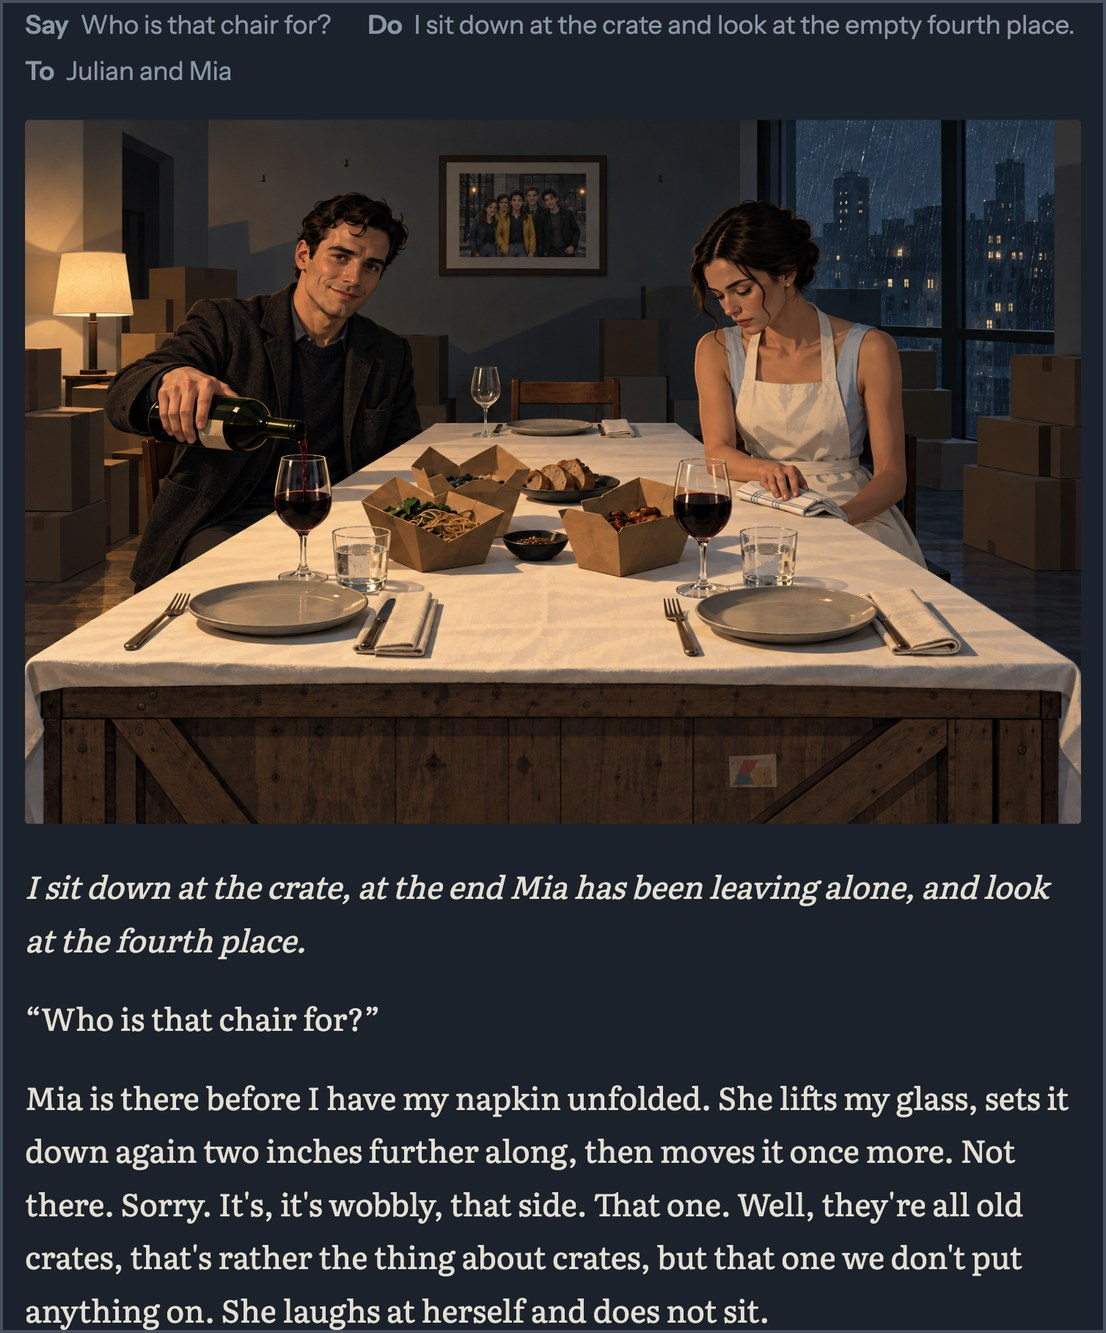
\includegraphics[width=\linewidth]{figures/play.jpg}\\[1mm]
  {\small (a) Play screen}
\end{minipage}\hfill
\begin{minipage}[c]{0.60\linewidth}
  \centering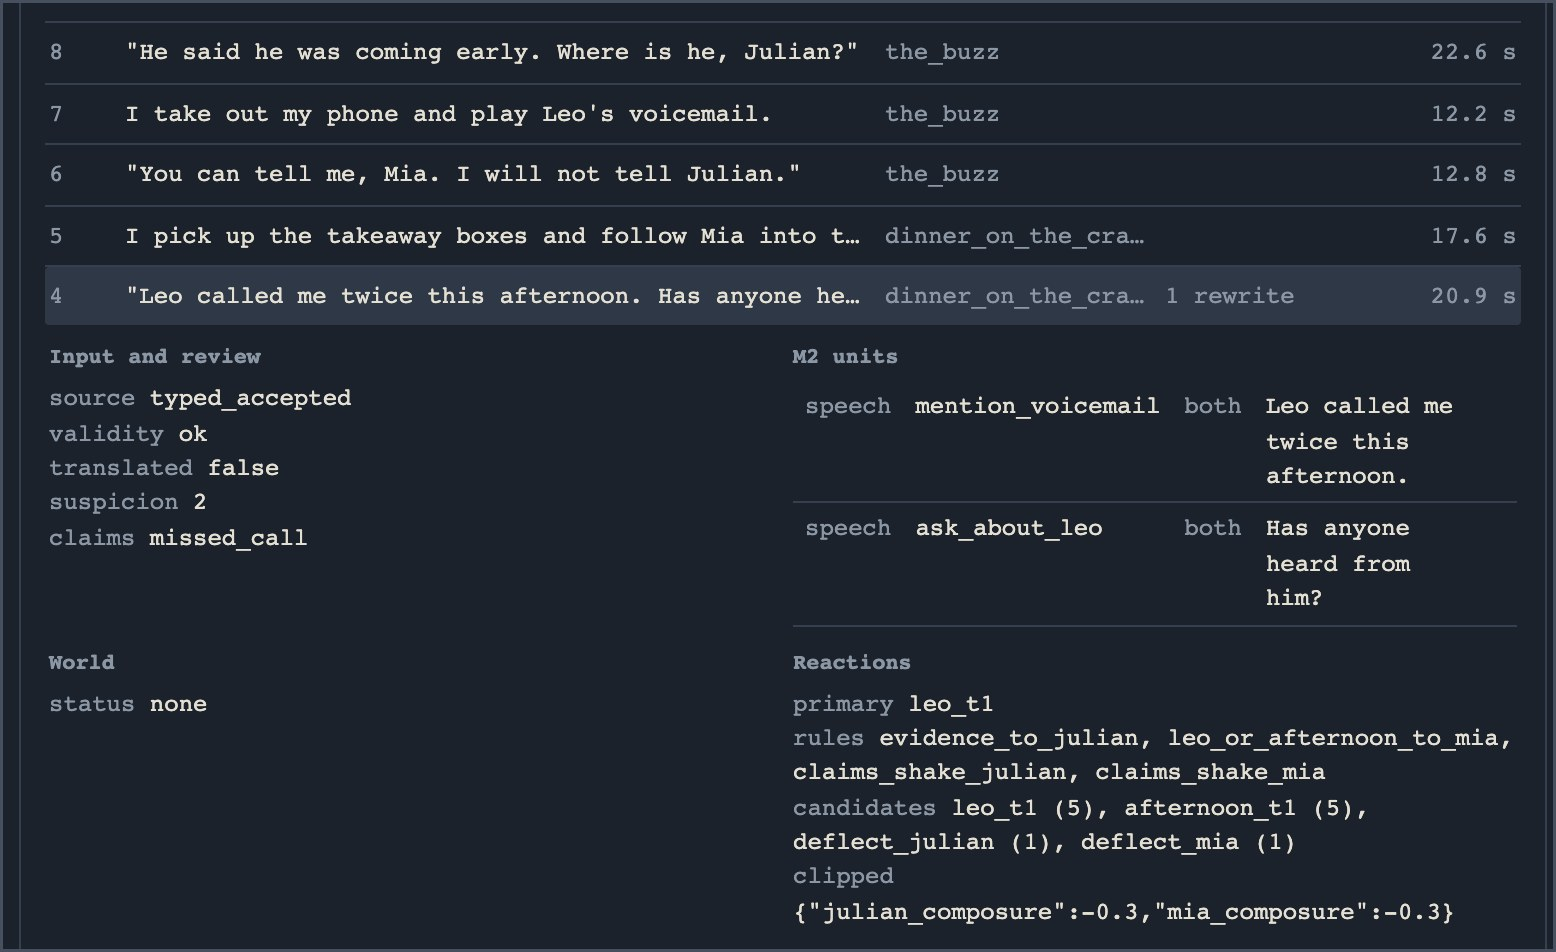
\includegraphics[width=\linewidth]{figures/console.jpg}\\[1mm]
  {\small (b) Developer Console}
\end{minipage}
\caption{The running system, from a live session with the real models (illustrations are AI-generated). (a) The player's line (here ``Who is that chair for?''), the inline illustration of the dinner on the crate, and the first-person passage that follows (the input box below it is cropped). (b) The Console on the same session: the turn list with the beat and latency of each turn, and the inspector for turn 4, showing the review result, the dialogue acts M2 extracted, the world result, and the reaction candidates with the chosen reaction.}
\label{fig:screens}
\end{figure}

\paragraph{Self-play data.}
\label{sec:data}
LLM players play whole sessions through the real engine. A persona is a HEXACO vector sampled from a multivariate normal with the published intercorrelations~\citep{moshagen2019hexaco}; 30\% of samples come from the tails and carry importance weights back to the population. Eight behaviour axes (curiosity, confrontation, verbosity, \dots) are noisy linear functions of the six domains, combined with a goal drawn from 32, a side, and a stance (report, cover, hesitate) that is only revealed to the player model after the truth comes out, so the card never hints at the plot. The model sees adjectives and three or four concrete rules, never numbers. Over 6{,}000 samples the weighted correlations stay within 0.022 of the published matrix. The player model rotates per session among DeepSeek flash, DeepSeek V4-pro, Kimi~K2.6, and Claude and GPT through their command lines; Kimi, Claude and GPT appear only in the test split so that M1 can be tested on player models it never saw. The narrator is fixed (DeepSeek flash) and the judge is a different family (Kimi~K3). The DM policy is mixed (LLM scorer 50\%, rule scorer 30\%, exploration 20\%) so that the logs contain non-greedy choices. A resumable, budget-capped runner logs every turn, decision, token count and cost, and a sharded workflow lets six people each run a slice of a fixed manifest, checked against a git tag.

\paragraph{Annotation protocol.}
Each beat choice depends on the story so far, so single decisions are not independent samples. Annotators see a \emph{state card}, a deterministic ledger of what has happened, and the turns of the current beat, but never what followed, and say which of two same-tier candidates is better (a \emph{prefix-blind} pairwise judgement). The budget is 250 judgements: 40 development, 100 test, 20 overlap, 30 optional branch probes, 20 whole-session reviews and 40 tension windows. The judge is calibrated on the development set and cross-checked by two other model families; agreement is reported with cluster-bootstrap intervals. No judgement has been collected yet.

\section{Initial results}
\label{sec:results}

\paragraph{Rule versus LLM paths (RQ1).}
Table~\ref{tab:modules} compares the two available paths on small hand-written sets (DeepSeek flash, prompt~v1, one run). The sets are small (10 to 35 items), so the numbers show direction, not significance.

\begin{table}[t]
\centering\small
\caption{Rule and LLM paths on hand-written evaluation sets.}
\label{tab:modules}
\begin{tabular}{llccc}
\toprule
Module & Metric & $n$ & Rule & LLM \\
\midrule
M2 review & validity accuracy / miss rate & 35 & 89\% / 17\% & \textbf{100\%} / \textbf{0\%} \\
M3 guard & accuracy / detection & 21 & 52\% / 57\% & \textbf{95\%} / \textbf{95\%} \\
M4 tension & MAE / Spearman & 10 & --- & 0.30 / 0.98 \\
M1 scorer & top-1 accuracy & 10 & 80\% & \textbf{100\%} \\
\bottomrule
\end{tabular}
\end{table}

\paragraph{Self-play dataset v0.}
Eleven complete sessions (8 from a pilot and 3 with Claude Opus 5.5 as the player) reached an ending (Table~\ref{tab:data}); two further pilot sessions whose player model was unusable (an expired login, an empty account balance) were detected and excluded, and the runner now aborts such sessions after three silent turns. Four of the five endings occurred (\texttt{second\_crate} did not); the sample is too small to compare player models. Latency is dominated by the narrator and guard: they take 92\% of server time, and a real player would wait a median of 10 s for the input review plus about 15 s for the passage.

\begin{table}[t]
\centering\small
\caption{Self-play dataset v0 (11 sessions, code before the fixes in Table~\ref{tab:issues}).}
\label{tab:data}
\begin{tabular}{lp{0.74\linewidth}}
\toprule
Players / DM & DeepSeek flash 4, DeepSeek pro 3, Claude Opus 5.5 3, GPT 1; LLM scorer 8, rule scorer 2, random 1 \\
Endings & \texttt{the\_witness} 3, \texttt{open\_it} 3, \texttt{confession} 3, \texttt{bon\_voyage} 2, \texttt{second\_crate} 0 \\
Length & 297 turns; mean 27 (12--36) per session \\
Cost, time, tokens & \$0.22 (0.12--0.31), 22 min (13--31), 0.67 M per session \\
Turn latency & median 17 s, mean 28 s, p90 68 s; narrator + guard 92\% \\
Input review & 13 of 310 attempts rejected (4.2\%); 17 of 21 deliberate rule-breaking inputs stopped \\
Guard, generation & 49 of 297 turns rewritten (16\%), 11 repaired (3.7\%); 9 ``new beat'' events, 29 distinct beats played \\
\bottomrule
\end{tabular}
\end{table}

\paragraph{The drama manager rarely has a real choice.}
Of 127 decisions, 50 were forced by the clock or a must-follow rule, 9 generated a new beat, 9 were endings, and only 59 were scored choices (Table~\ref{tab:dm}). A scored decision has 2.4 candidates on average, but one of them is the generate option, so there are only 1.5 authored candidates, and only 25 of 59 (42\%) offer two or more. With the LLM scorer the top candidate has a median probability of 0.99 and is chosen in 46 of 48 decisions, because the model gives one beat 6 or 7 points and the rest near zero. Sampling temperature therefore cannot supply diversity. Preference pairs for M1 depend on the number of eligible beats, which is a property of the pool and the preconditions, not of the sampler. This pushes us toward a larger pool, higher-temperature exploration policies, and pairing generated beats with authored ones.

\begin{table}[t]
\centering\small
\caption{Scored beat decisions by policy. Candidates in brackets exclude the generate option.}
\label{tab:dm}
\begin{tabular}{lccccc}
\toprule
Policy & $n$ & Candidates & Median max $p$ & $\max p>0.9$ & $\ge 2$ authored \\
\midrule
LLM scorer, $\tau{=}1$ & 48 & 2.42 (1.42) & 0.988 & 37 & 19 \\
Rule scorer & 10 & 2.50 (1.60) & 0.826 & 3 & 5 \\
All (incl.\ 1 random) & 59 & 2.44 (1.46) & 0.984 & 40 & 25 \\
\bottomrule
\end{tabular}
\end{table}

\paragraph{Tension.}
Figure~\ref{fig:tension} compares the target arc, the tension each beat declares, and M4's reading of the text (116 estimates). The mean distance from the target is 1.05 points (0.38--1.72 per session). The text reads about 0.8 points more tense than the beats declare, and it is already near 3 in the first two minutes, where the target is 1. The scorer sees the declared value, so it works with a picture that is lower than what the reader gets. Either the narrator's opening cues (cold hands, a corner wiped over and over) are too heavy, or the target arc should change.

\begin{figure}[t]
\centering
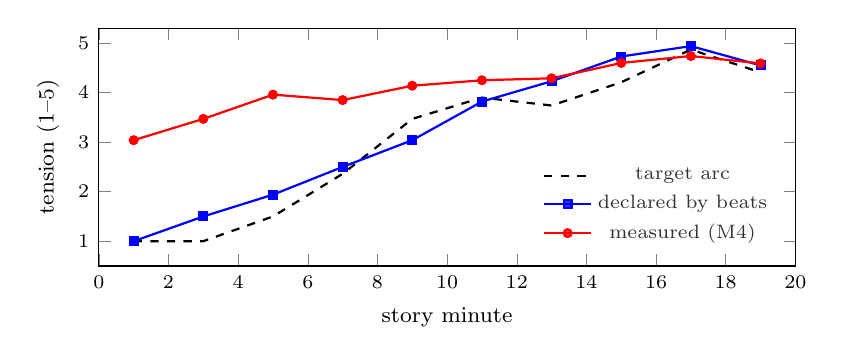
\begin{tikzpicture}
\begin{axis}[width=0.86\linewidth,height=4.6cm,xlabel={story minute},ylabel={tension (1--5)},xmin=0,xmax=20,ymin=0.5,ymax=5.3,ytick={1,2,3,4,5},
  legend style={font=\scriptsize,at={(0.98,0.05)},anchor=south east,draw=none,fill=white,fill opacity=0.8},
  tick label style={font=\scriptsize},label style={font=\footnotesize}]
\addplot[black,dashed,thick] coordinates {(1,1.00)(3,1.00)(5,1.50)(7,2.36)(9,3.47)(11,3.90)(13,3.74)(15,4.21)(17,4.87)(19,4.41)};
\addplot[blue,mark=square*,mark size=1.4pt,thick] coordinates {(1,1.00)(3,1.50)(5,1.94)(7,2.50)(9,3.04)(11,3.82)(13,4.23)(15,4.73)(17,4.94)(19,4.55)};
\addplot[red,mark=*,mark size=1.4pt,thick] coordinates {(1,3.04)(3,3.47)(5,3.96)(7,3.85)(9,4.14)(11,4.25)(13,4.29)(15,4.60)(17,4.74)(19,4.59)};
\legend{target arc,declared by beats,measured (M4)}
\end{axis}
\end{tikzpicture}
\caption{Mean tension by story minute over 11 sessions: the target arc, the value each beat declares, and M4's estimate. Each point averages 9 to 16 estimates.}
\label{fig:tension}
\end{figure}

\paragraph{What reading the transcripts showed.}
Counts alone hid several problems, so we read all eight pilot transcripts line by line (Table~\ref{tab:issues}). The clearest case: in the arrival beat, Mia asked ``Did you come by car?'' twice in 6 of the 8 sessions that opened with the arrival beat (one of them an Opus session), even after the player had answered. The opening passage has no step to follow, so the narrator spent her character tell there, and the beat's own step played the same line again. We stopped handing character tells to the opening passage and made the step conditional on a new state variable that records which habits the narration has used. With the live narrator, 7 of 8 openings asked about the car before the change and 0 of 8 after; in two full sessions the question was asked once. A second fix, a per-habit use budget, did \emph{not} lower how often Mia wipes the same clean corner in two validation sessions (12 to 8, and 7 to 12 mentions): about half the mentions come from authored beat or reaction text, and the rest from the character's surface description and the narrator copying its recent passages. We report this negative result and treat it as open.

\begin{table}[t]
\centering\small
\caption{Problems found by reading the pilot transcripts.}
\label{tab:issues}
\begin{tabular}{p{0.37\linewidth}p{0.33\linewidth}p{0.20\linewidth}}
\toprule
Finding & Cause & Status \\
\midrule
Arrival question asked twice (6 of 8 sessions) & Tell used in the opening; step repeats it & Fixed: 7/8 $\to$ 0/8 \\
``Clean corner'' recurs 3--20 times per session & Authored text, character summary, imitation & Budget added, no effect \\
Scripted lines ignore the player; 34 lines recur in $\ge$3 sessions (33\% of NPC speech) & Step text is fixed; words select the outcome only & Open; planned \\
Covering up recorded as truth or lost (3 of 3 ``cover'' players) & \texttt{nora\_told} tracks factual truth; the last turn can overwrite it & Open; planned \\
Stated intent delayed (answering the door: 6+ attempts, 14 turns) & Stalling reactions are unlimited & Open; planned \\
Random policy picks ``don't go yet'' as first beat & Preconditions allow it at turn 0 & Open; planned \\
\bottomrule
\end{tabular}
\end{table}

The third row matters most for the drama manager. After a player told Nora that Leo was dead, she still asked whether he was with them (excerpt from pilot session 6):
\begin{quote}\small
\textbf{Player:} Nora---call the police. Leo's dead. He's here, at Julian's. Tell them to come now.\\
\textbf{Julian:} Who's texting you, Ryan?\\
\textbf{Nora (next turn):} Is Leo with you? He said he'd be at Julian's tonight with you. He's not picking up.
\end{quote}
Such lines are authored beat text: the player's words pick the branch, not the wording. This matters for learning, because annotators judge a beat choice by how the scene reads afterwards, and a scene that ignores the player cannot show whether the choice fit.

\paragraph{Input understanding (M2) (RQ3).}
M2 is being distilled into one multilingual encoder, mDeBERTa-v3~\citep{he2023debertav3}, with heads for segmentation (per token), act, topics, action verb and target (per unit), and addressee, suspicion, claims and two answer types (per turn). Labels come from the LLM teacher on self-play turns, and results are scored on a frozen test split (\texttt{test\_v1}) against a ladder of baselines: keyword rules (rung~0), TF-IDF with logistic regression (rung~1), frozen multilingual sentence embeddings (rung~2), and the multi-head model (rung~4). Table~\ref{tab:m2} is awaiting the numbers; a first observation from the training logs is that turn-level heads reading only the [CLS] vector trail the frozen-embedding baseline while the mean-pooled unit heads beat it \todo{M2 owner: confirm with numbers}.

\begin{table}[t]
\centering\small
\caption{Input understanding on the frozen test split. \todo{M2 owner to fill every cell from the CARC runs; add the teacher's self-agreement as an upper bound and the number of games and turns behind each split.}}
\label{tab:m2}
\setlength{\tabcolsep}{3pt}
\begin{tabular}{lccccc}
\toprule
System & Acts $\mu$F1 & Topics $\mu$F1 & Addr.\ acc & Nora acc & Seg.\ F1 \\
\midrule
Rung 0 (rules / majority) & \todo{} & \todo{} & \todo{} & \todo{} & \todo{} \\
Rung 1 (TF-IDF + LR) & \todo{} & \todo{} & \todo{} & \todo{} & \todo{} \\
Rung 2 (frozen embeddings + LR) & \todo{} & \todo{} & \todo{} & \todo{} & \todo{} \\
Rung 4 (multi-head mDeBERTa) & \todo{} & \todo{} & \todo{} & \todo{} & \todo{} \\
Teacher self-agreement & \todo{} & \todo{} & \todo{} & \todo{} & \todo{} \\
\bottomrule
\end{tabular}
\end{table}

\paragraph{Beat scoring (M1) (RQ2).}
There is no trained scorer yet. It is blocked by labels: the annotation tool and the first judgements, and the judge calibration, come before any training, and the thin candidate sets above limit how many informative pairs a session yields. What exists is the part that makes training possible: every decision is logged with its state, all candidates, their scores and probabilities, so that offline policy evaluation and pairwise labelling can be run later; and the rule and LLM scorers give two baselines for the comparison.

\section{Updated plan}
\label{sec:plan}

We are about two weeks behind the original schedule, mainly because the engine and the data pipeline took longer than planned. Table~\ref{tab:plan} is the plan to the poster session on November~30, ordered by what each step unblocks.

\begin{table}[t]
\centering\small
\caption{Plan to the poster session (dates are targets).}
\label{tab:plan}
\begin{tabular}{p{0.17\linewidth}p{0.75\linewidth}}
\toprule
Dates & Work \\
\midrule
Nov 16--18 & Fix beat text that ignores disclosures and the \texttt{nora\_told} semantics; random policy skips the opening; first 30-session round on six machines (about \$7). \\
Nov 16--21 & Annotation packet generator; 140 development and test judgements; M2 ablations over seeds. \\
Nov 19--23 & Calibrate the judge against humans; go/no-go for synthetic labels. \\
Nov 21--26 & Second self-play round (about 100 sessions); train M1 on judge labels; compare with the rule and LLM scorers on the human test set and unseen player models. \\
Nov 26--29 & Poster: Console screenshots, tension curves, live demo hardening. \\
\bottomrule
\end{tabular}
\end{table}

\textbf{Cut or reduced.} The user study, extending the pool beyond about 30 beats, trained M3 and M4, and the earlier 2D portrait layer are dropped; the pool will grow only as far as M1 data requires. \textbf{Risks.} (1) The judge may disagree with humans; then M1 can train only on the human labels, which are too few for a neural scorer, and we would fall back to a linear scorer over beat features. (2) Thin candidate sets limit informative pairs; we raise exploration and pair generated beats with authored ones. (3) Time: the plan assumes the first human labels exist by November~21.

\bibliographystyle{plainnat}
\bibliography{refs}

\end{document}
